\documentclass[tikz,border=5mm]{standalone}
\usepackage{amsmath}
\usepackage{amsfonts} % For \infty
\usepackage{xcolor}

\usetikzlibrary{positioning, arrows.meta, matrix, calc}

% Define custom colors
\definecolor{orange_main}{HTML}{FF8800}
\definecolor{beige_bg}{HTML}{FFF5EC} % A soft, light beige
\definecolor{line_color}{HTML}{555555} % Dark gray for lines

\begin{document}

% Title block
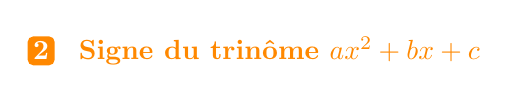
\begin{tikzpicture}[baseline=(N.south west)]
    \node[fill=orange_main, text=white, rectangle, rounded corners=2pt, inner sep=2pt, font=\bfseries] (N) {2};
    \node[right=5pt of N, anchor=west] {\textbf{\color{orange_main} Signe du trinôme $ax^2 + bx + c$}};
\end{tikzpicture}
\vspace{1em} % Small vertical space after title

\begin{tikzpicture}[
    % Global settings for node distances and arrow style
    node distance=1.2cm and 2cm, % Vertical and horizontal distance
    arrow_style/.style={-Latex, thick, line_color},
    % Styles for flowchart blocks
    block/.style={
        rectangle,
        draw=orange_main,
        thick,
        fill=beige_bg,
        inner xsep=8pt,
        inner ysep=5pt,
        text depth=0.8ex, % Ensure consistent baseline for math
        text height=1.5ex,
    },
    math_block/.style={
        block,
        font=\bfseries, % Make math bold too
    },
    % Styles for table cells within matrices
    tabcell/.style={
        rectangle,
        draw=none, % No individual cell draw, matrix will draw outer border and internal lines
        fill=beige_bg,
        minimum height=1.8em,
        inner sep=2pt,
        align=center,
        font=\sffamily\small,
        text depth=0.5ex, text height=1em, % Consistent height for text in cells
    },
    tabhead/.style={tabcell, text width=1.5em}, % Style for x and P(x) labels
    tabval/.style={tabcell, text width=4em}, % Style for values like -infty, x0, +infty
    zero_text/.style={font=\sffamily\small, anchor=center, inner sep=0pt, fill=beige_bg}, % Style for the '0' label
]

% Flowchart Nodes
\node[block] (Px) {$P(x) = ax^2 + bx + c$};
\node[math_block, below=1.5cm of Px] (Delta) {$\Delta = b^2 - 4ac$};

% Conditional Delta nodes
\node[math_block, below left=1.5cm and 3cm of Delta] (Delta_lt0) {$\Delta < 0$};
\node[math_block, below=1.5cm of Delta] (Delta_eq0) {$\Delta = 0$};
\node[math_block, below right=1.5cm and 3cm of Delta] (Delta_gt0) {$\Delta > 0$};

% Flowchart Arrows
\draw[arrow_style] (Px) -- (Delta);

% Split arrows from Delta to conditional nodes
\coordinate (h_split) at ([yshift=-0.75cm]Delta.south); % Horizontal split point below Delta
\draw[arrow_style] (Delta.south) -- (h_split);
\draw[arrow_style] (h_split) -| (Delta_lt0.north);
\draw[arrow_style] (h_split) -| (Delta_eq0.north);
\draw[arrow_style] (h_split) -| (Delta_gt0.north);

% --- Tables for each case ---

% Table 1: Delta < 0
\matrix (table1) [
    matrix of nodes,
    nodes=tabcell,
    row sep=-\pgflinewidth, column sep=-\pgflinewidth,
    below=1cm of Delta_lt0,
    % Define column styles and node names for easier referencing
    column 1/.style={nodes={tabhead}},
    column 2/.style={nodes={tabval}},
    column 3/.style={nodes={tabval}},
]
{
    $x$ & $-\infty$ & $+\infty$ \\
    $P(x)$ & & \\
};
% Draw outer and inner lines for Table 1
\draw[line_color, thick] (table1.north west) rectangle (table1.south east); % Outer box
\draw[line_color, thick] (table1-1-1.south) -- (table1-1-3.south); % Horizontal line under first row
\draw[line_color, thick] (table1-1-1.east) -- (table1-2-1.east); % Vertical line after first column
% Overlay spanning node for Table 1
\node[tabcell, text width=8em] at ($(table1-2-2.center)!0.5!(table1-2-3.center)$) {Signe de a};

% Table 2: Delta = 0
\matrix (table2) [
    matrix of nodes,
    nodes=tabcell,
    row sep=-\pgflinewidth, column sep=-\pgflinewidth,
    below=1cm of Delta_eq0,
    % Define column styles and node names
    column 1/.style={nodes={tabhead}},
    column 2/.style={nodes={tabval}},
    column 3/.style={nodes={tabval}},
    column 4/.style={nodes={tabval}},
]
{
    $x$ & $-\infty$ & $x_0$ & $+\infty$ \\
    $P(x)$ & Signe de a & & Signe de a \\
};
% Draw outer and inner lines for Table 2
\draw[line_color, thick] (table2.north west) rectangle (table2.south east); % Outer box
\draw[line_color, thick] (table2-1-1.south) -- (table2-1-4.south); % Horizontal line under first row
\draw[line_color, thick] (table2-1-1.east) -- (table2-2-1.east); % Vertical line after first column
\draw[line_color, thick] (table2-1-2.east) -- (table2-2-2.east); % Vertical line after -infty
\draw[line_color, thick] (table2-1-3.east) -- (table2-2-3.east); % Vertical line after x_0
% Place the '0' on the vertical line
\node[zero_text] at (table2-1-3.east |- table2-2-3.center) {$0$};

% Table 3: Delta > 0
\matrix (table3) [
    matrix of nodes,
    nodes=tabcell,
    row sep=-\pgflinewidth, column sep=-\pgflinewidth,
    below=1cm of Delta_gt0,
    % Define column styles and node names
    column 1/.style={nodes={tabhead}},
    column 2/.style={nodes={tabval}},
    column 3/.style={nodes={tabval}},
    column 4/.style={nodes={tabval}},
    column 5/.style={nodes={tabval}},
    column 6/.style={nodes={tabval}},
]
{
    $x$ & $-\infty$ & $x_1$ & & $x_2$ & $+\infty$ \\
    $P(x)$ & Signe de a & & Signe de -a & & Signe de a \\
};
% Draw outer and inner lines for Table 3
\draw[line_color, thick] (table3.north west) rectangle (table3.south east); % Outer box
\draw[line_color, thick] (table3-1-1.south) -- (table3-1-6.south); % Horizontal line under first row
\draw[line_color, thick] (table3-1-1.east) -- (table3-2-1.east); % Vertical line after first column
\draw[line_color, thick] (table3-1-2.east) -- (table3-2-2.east); % Vertical line after -infty
\draw[line_color, thick] (table3-1-3.east) -- (table3-2-3.east); % Vertical line after x_1
\draw[line_color, thick] (table3-1-5.east) -- (table3-2-5.east); % Vertical line after x_2
% Place the '0's on the vertical lines
\node[zero_text] at (table3-1-3.east |- table3-2-3.center) {$0$};
\node[zero_text] at (table3-1-5.east |- table3-2-5.center) {$0$};

\end{tikzpicture}

\end{document}
